\level{2}{APotiSwitch}

\level{3}{Structure}
{
\centering{}
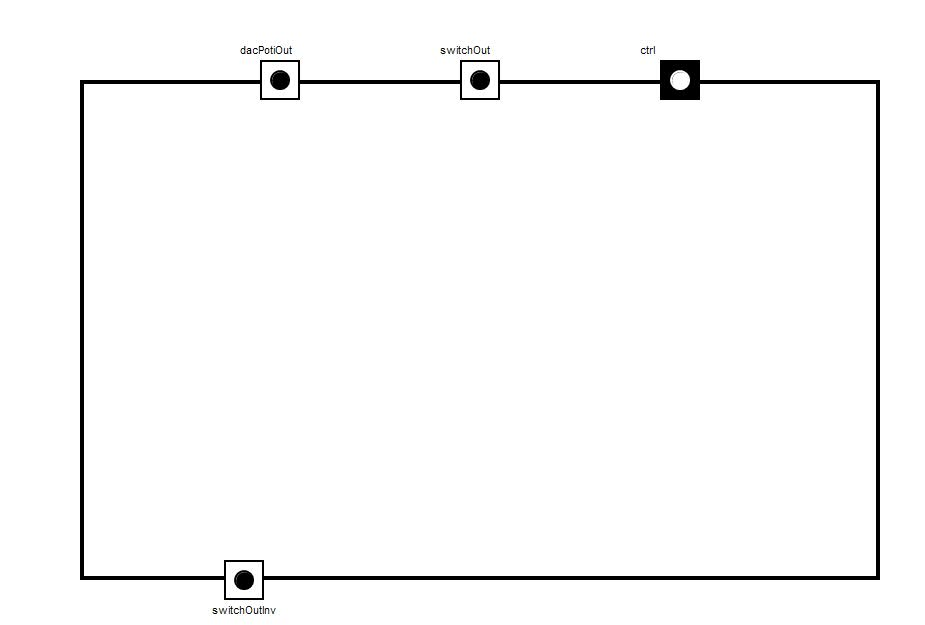
\includegraphics[width=1.0\textwidth]{./images/APotiSwitch_structure.jpg}
\figcaption{APotiSwitch Structure}
}

\level{3}{Ports}
\begin{tabular}[ht]{|l|l|l|l|l|p{5cm}|}
\hline
\textbf{Name} & \textbf{Protocol} & \textbf{Type} & \textbf{Kind} & \textbf{Multiplicity} & \textbf{Description}\\
\hline
dacPotiOut & PDac & conj. & external & 1 & \\
\hline
switchOut & POnOff & conj. & external & 1 & \\
\hline
ctrl & PPotiSwitchControl & reg. & external & 1 & \\
\hline
switchOutInv & POnOff & conj. & external & 1 & \\
\hline
\end{tabular}

\level{3}{Behavior}
\level{4}{Top Level}
{
\centering{}
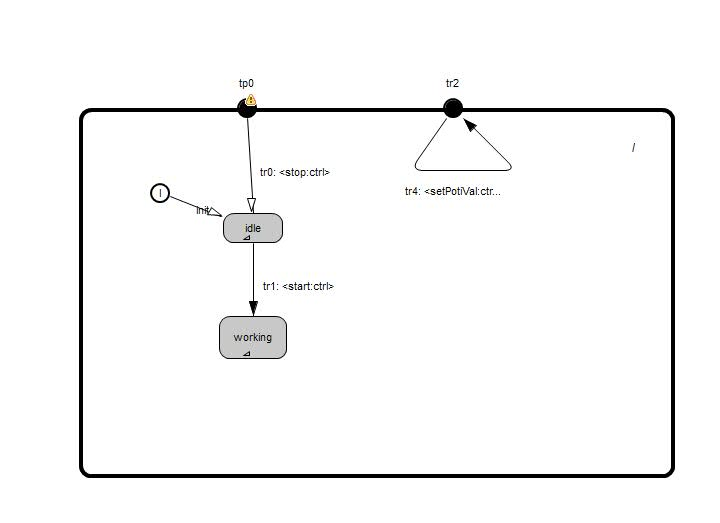
\includegraphics[width=1.0\textwidth]{./images/APotiSwitch_behavior.jpg}
\figcaption{APotiSwitch Top State}
}

\begin{par}

\end{par}


\level{3}{Attributes}
\begin{tabular}[ht]{|l|l|p{8cm}|}
\hline
\textbf{Name} & \textbf{Type} & \textbf{Description}\\
\hline
actualOutVal & uint32 & \\
\hline
\end{tabular}

